\documentclass[border=4pt]{standalone}
\usepackage{fontspec}
\usepackage{amsmath}
\usepackage{unicode-math}
\setmainfont{Latin Modern Roman}
\setmathfont{Latin Modern Math}
\usepackage{pgfplots}
\usepackage{pgfplotstable}
\pgfplotsset{compat=1.18}
\usepackage{tkz-euclide}
\usetikzlibrary{arrows.meta,calc,angles,quotes,patterns,3d,backgrounds}
\definecolor{ink}{HTML}{123428}
\definecolor{asy}{HTML}{475569}
\definecolor{mint}{HTML}{86e0bd}
\tikzset{asym/.style={asy, line width=0.9pt, dash pattern=on 5pt off 3.5pt},
         guide/.style={gray!70, line width=0.6pt, densely dotted},
         dot/.style={circle, inner sep=0pt, minimum size=5pt, draw=white, line width=0.5pt},
         odot/.style={circle, inner sep=0pt, minimum size=5.5pt, fill=white, line width=1pt},
         lab/.style={font=\footnotesize, inner sep=1.5pt, text=ink}}
\begin{document}
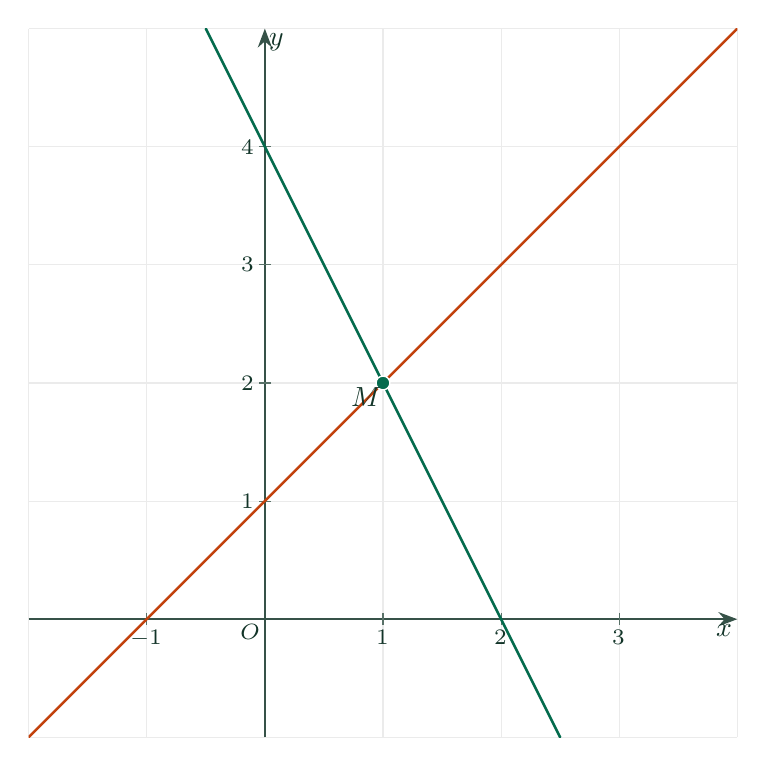
\begin{tikzpicture}[x=1.5000cm, y=1.5000cm]
\draw[gray!16, line width=0.4pt] (-2,-1) -- (-2,5) (-1,-1) -- (-1,5) (0,-1) -- (0,5) (1,-1) -- (1,5) (2,-1) -- (2,5) (3,-1) -- (3,5) (4,-1) -- (4,5);
\draw[gray!16, line width=0.4pt] (-2,-1) -- (4,-1) (-2,0) -- (4,0) (-2,1) -- (4,1) (-2,2) -- (4,2) (-2,3) -- (4,3) (-2,4) -- (4,4) (-2,5) -- (4,5);
\draw[ink!85, line width=0.7pt, -{Stealth[length=2.4mm]}] (-2,0) -- (4,0) node[anchor=north east, lab, font=\normalsize] {$x$};
\draw[ink!85, line width=0.7pt, -{Stealth[length=2.4mm]}] (0,-1) -- (0,5) node[anchor=north west, lab, font=\normalsize] {$y$};
\draw[ink!70] (-1,0.05333333333333334) -- (-1,-0.05333333333333334) node[below, lab, font=\footnotesize] {$-1$};
\draw[ink!70] (1,0.05333333333333334) -- (1,-0.05333333333333334) node[below, lab, font=\footnotesize] {$1$};
\draw[ink!70] (2,0.05333333333333334) -- (2,-0.05333333333333334) node[below, lab, font=\footnotesize] {$2$};
\draw[ink!70] (3,0.05333333333333334) -- (3,-0.05333333333333334) node[below, lab, font=\footnotesize] {$3$};
\draw[ink!70] (0.05333333333333334,1) -- (-0.05333333333333334,1) node[left, lab, font=\footnotesize] {$1$};
\draw[ink!70] (0.05333333333333334,2) -- (-0.05333333333333334,2) node[left, lab, font=\footnotesize] {$2$};
\draw[ink!70] (0.05333333333333334,3) -- (-0.05333333333333334,3) node[left, lab, font=\footnotesize] {$3$};
\draw[ink!70] (0.05333333333333334,4) -- (-0.05333333333333334,4) node[left, lab, font=\footnotesize] {$4$};
\node[lab, anchor=north east] at (0,0) {$O$};
\tkzDefPoint(-0.5,5){tmp1}
\tkzDefPoint(2.5,-1){tmp2}
\tkzDefPoint(4,5){tmp3}
\tkzDefPoint(-2,-1){tmp4}
\tkzDefPoint(1,2){M}
\begin{scope}
\clip (-2,-1) rectangle (4,5);
\tkzDrawSegment[draw={rgb,255:red,4;green,107;blue,77}, line width=0.90pt](tmp1,tmp2)
\tkzDrawSegment[draw={rgb,255:red,194;green,65;blue,12}, line width=0.90pt](tmp3,tmp4)
\end{scope}
\node[dot, fill={rgb,255:red,4;green,107;blue,77}] at (M) {};
\node[lab, font=\normalsize, anchor=north east] at (1,2) {$M$};
\end{tikzpicture}
\end{document}
